\mychapter{4}{MultiVariate Analysis}
\label{sec:unchapitre}

%\section{Boosted Decision Tree}

Now that we get background and signal samples we can perform the MVA for classification.\\
For this work the TMVA framework from ROOT was used. Multiple MVA were tested (fig. \ref{mva_multiple}) with default configuration then the 2
bests were selected for the tuning of their parameters.\\

\begin{figure}[h!]
\centering
    \begin{subfigure}[h!]{0.4\textwidth}
    \centering
        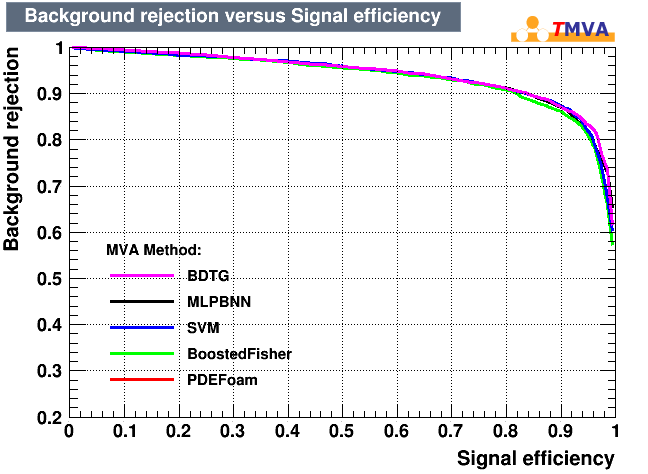
\includegraphics[width=\textwidth]{mva_multiple}
        \caption{ROC curve for the 5 bests MVA that has been tested.}
        \label{mva_multiple}
  \end{subfigure}
  ~
    \begin{subfigure}[h!]{0.4\textwidth}
    \centering
        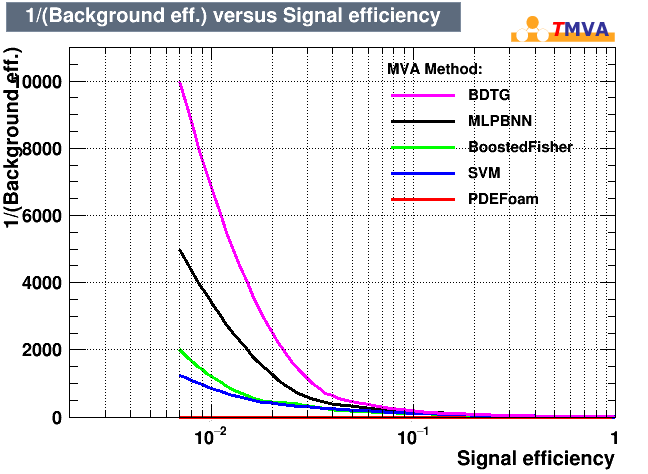
\includegraphics[width=\textwidth]{inv_mva_multiple.png}
        \caption{Inverse ROC curve for the 5 bests MVA that has been tested.}
        \label{inv_mva_multiple}
  \end{subfigure}
\end{figure}


\section{Artificial Neural Network}


Input variable optimization






%%% Local Variables: 
%%% mode: latex
%%% TeX-master: "isae-report-template"
%%% End: 
